\section{Problems}

\frame{\frametitle{GAN: Problems}
	\vspace{-1cm}
	\begin{itemize}
		\item Many GAN models suffer the following major problems:
		      \begin{itemize}
			      \item \alert{Mode collapse:} the generator collapses which produces limited varieties of samples
			      \item \alert{Non-convergence:} the model parameters oscillate, destabilize and never converge
			      \item \alert{Diminished gradient:} he discriminator gets too successful that the generator gradient vanishes and learns nothing
			      \item Unbalance between the generator and discriminator causing overfitting
			      \item Highly sensitive to the hyperparameter selections.
		      \end{itemize}
	\end{itemize}
}

\frame{\frametitle{Mode Collapse}
	\begin{itemize}
		\item Real-life data distributions are multimodal.
		\item In MNIST, there are 10 major modes from digit ‘0’ to digit ‘9’.
		\item The samples below are generated by two different GANs.
		\item We can see the generator creates a single mode only. This is called mode collapse.
	\end{itemize}
	\hyperlink{Unrolled}{
		\begin{figure}
			\centering
			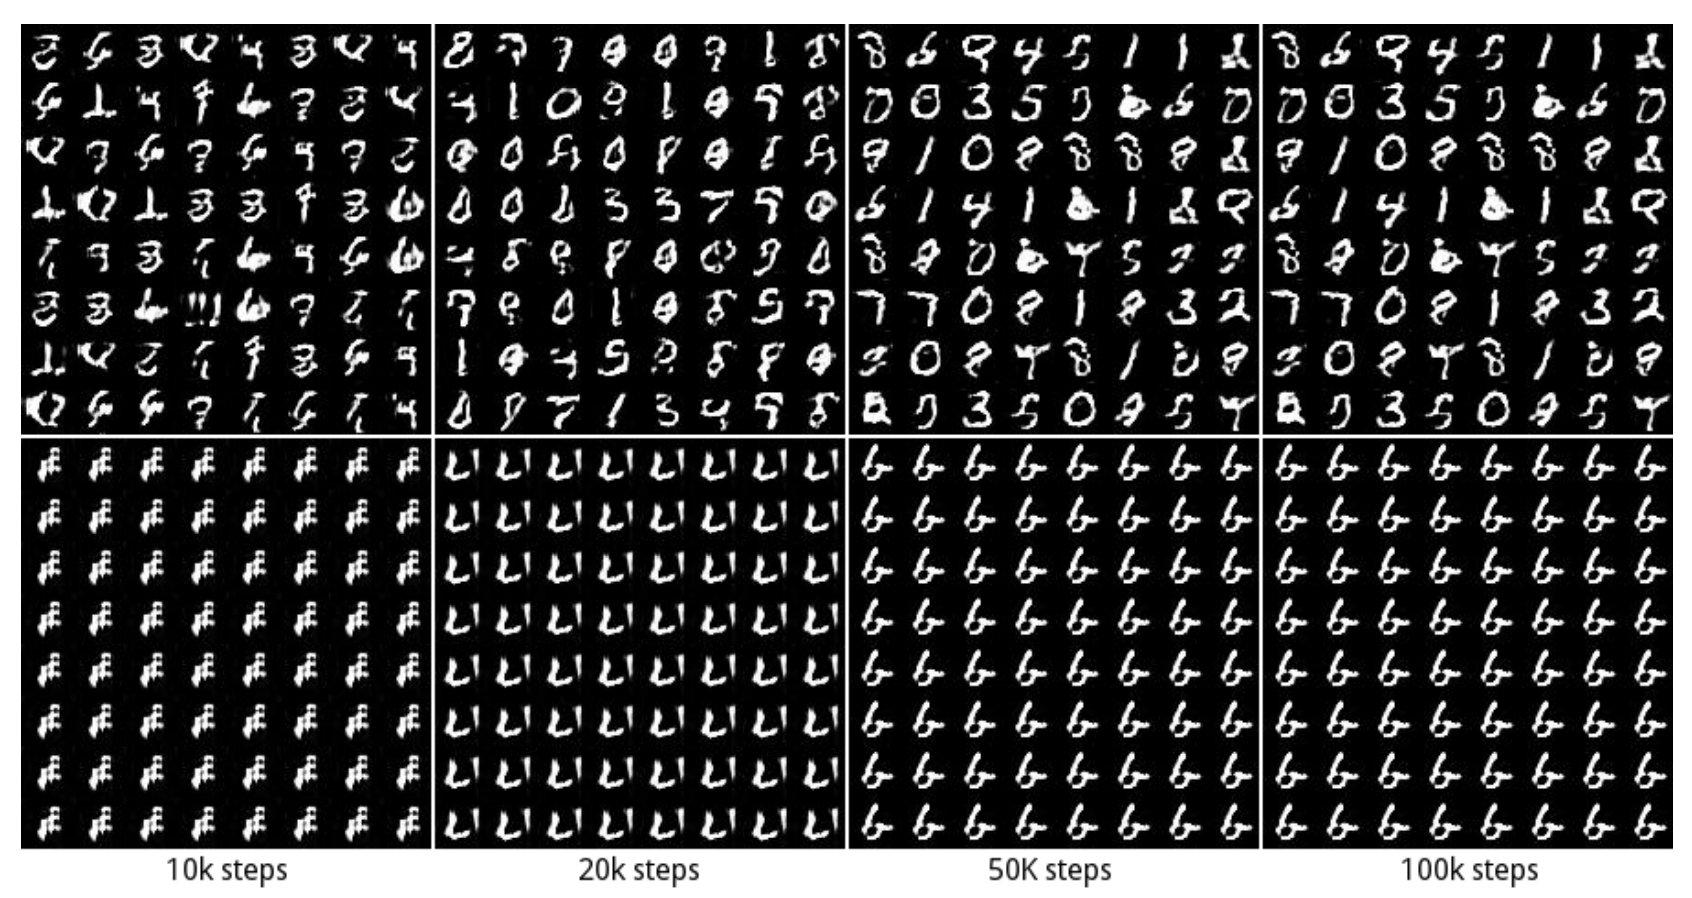
\includegraphics[width=8cm]{Unrolled}
			\caption{GAN mode collapse \href{https://arxiv.org/abs/1611.02163}{(Source)}}
		\end{figure}
	}
}

\frame{\frametitle{Why Mode Collapse in GAN?}
	\begin{itemize}
		\item The images below with the same underlined color look similar and the mode starts collapsing.
	\end{itemize}
	\hyperlink{Mode1}{
		\begin{figure}
			\centering
			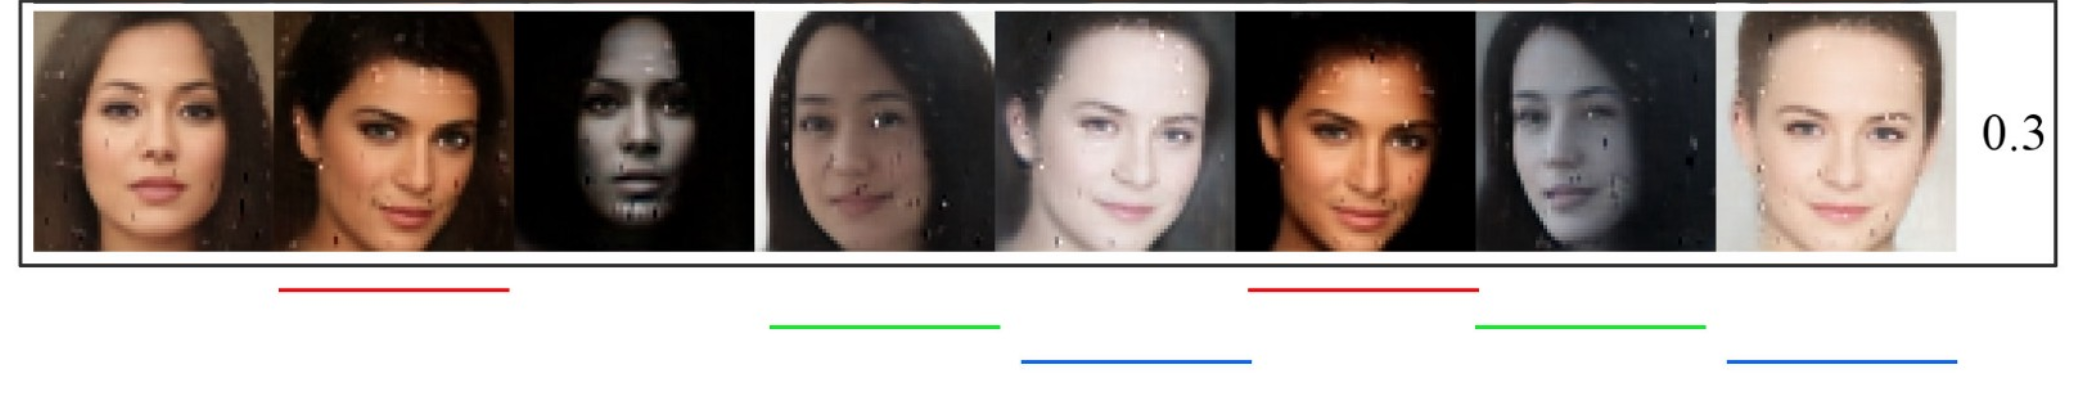
\includegraphics[width=9cm]{Mode1}
			\caption{Modified from \href{https://towardsdatascience.com/gan-ways-to-improve-gan-performance-acf37f9f59b}{(Source)}}
		\end{figure}
	}
	\begin{itemize}
		\item Let’s see how it may occur. The objective of the GAN generator is to create images that can fool the discriminator D the most.
	\end{itemize}
	\begin{figure}
		\centering
		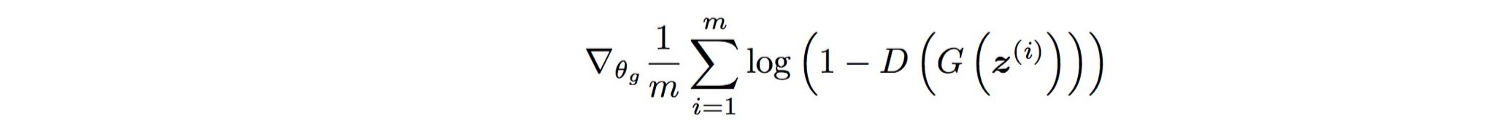
\includegraphics[width=10cm]{mode2}
	\end{figure}
	\begin{itemize}
		\item But let’s consider one extreme case where G is trained extensively without updates to D.

	\end{itemize}
}

\frame{\frametitle{Why Mode Collapse in GAN?}
	\begin{itemize}
		\item The generated images will converge to find the optimal image $x*$ that fool $D$ the most, the most realistic image from the discriminator perspective.
		\item In this extreme, x* will be independent of z.
	\end{itemize}
	\begin{figure}
		\centering
		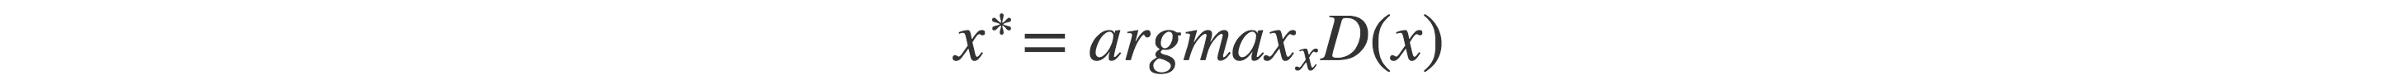
\includegraphics[width=10cm]{mode3}
	\end{figure}
	\begin{itemize}
		\item The mode collapses to a single point.
		\item The gradient associated with z approaches zero.
	\end{itemize}
	\begin{figure}
		\centering
		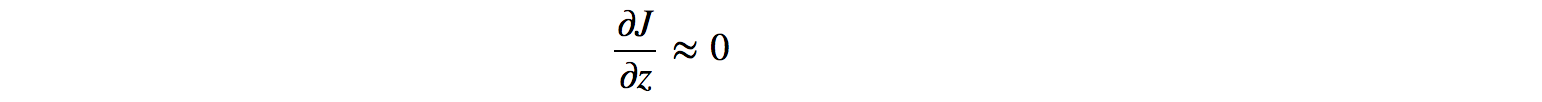
\includegraphics[width=10cm]{mode4}
	\end{figure}
	\begin{itemize}
		\item Solution?
		\item Unrolled GAN
	\end{itemize}
	\hyperlink{Unrolled}{
		\begin{figure}
			\centering
			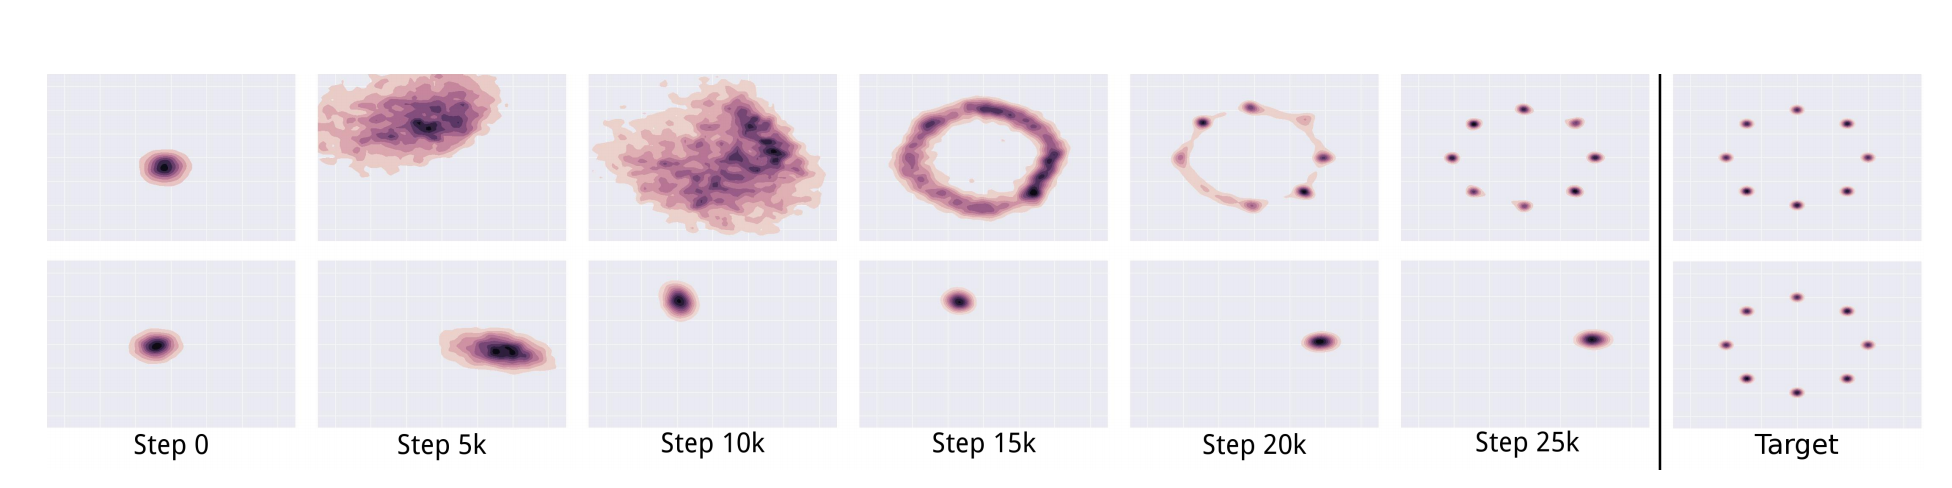
\includegraphics[width=9cm]{Unrolled2}
			\caption{ Unrolled GAN vs Vanilla GAN \href{https://arxiv.org/abs/1611.02163}{(Source)}}
		\end{figure}
	}
}

\frame{\frametitle{Nash Equilibrium}
	\begin{itemize}
		\item GAN is based on the zero-sum non-cooperative game.
		\item A zero-sum game is also called \alert{minimax}.
		\item In game theory, the GAN model converges when the discriminator and the generator reach a \alert{Nash equilibrium}
	\end{itemize}
	\begin{figure}
		\centering
		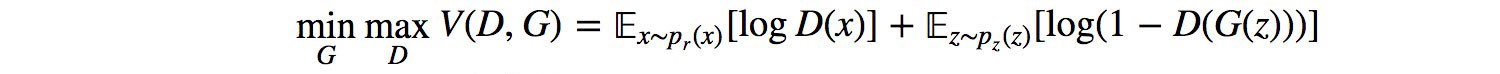
\includegraphics[width=10cm]{minmax}
	\end{figure}
	\begin{itemize}
		\item Nash equilibrium happens when one player will not change its action regardless of what the opponent may do.
		\item Consider two player A and B which control the value of x and y respectively. Player A wants to maximize the value xy while B wants to minimize it.
	\end{itemize}
	\begin{figure}
		\centering
		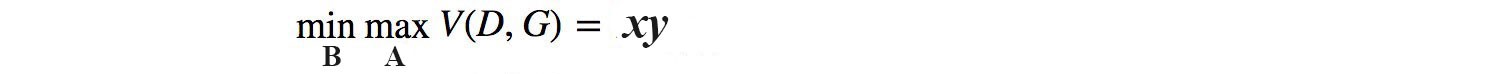
\includegraphics[width=10cm]{minmax2}
	\end{figure}
	\begin{itemize}
		\item The Nash equilibrium is $x = y =0$
		\item This is the only state where the action of your opponent does not matter. It is the only state that any opponents’ actions will not change the game outcome.
	\end{itemize}
}

\frame{\frametitle{Non-convergence}
	\begin{itemize}
		\item Let’s see whether we can find the Nash equilibrium easily using the gradient descent.
		\item We update the parameter x and y based on the gradient of the value function V.
	\end{itemize}
	\begin{figure}
		\centering
		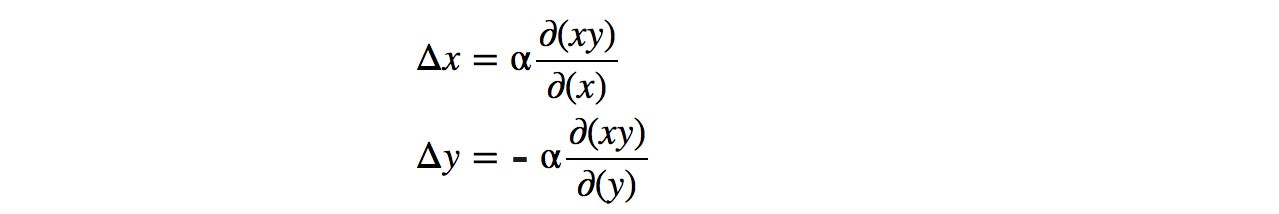
\includegraphics[width=7cm]{minmax3}
	\end{figure}
	\begin{itemize}
		\item Where α is the learning rate. When we plot x, y, and xy against the training iterations, we realize our solution does not converge.
	\end{itemize}
	\begin{figure}
		\centering
		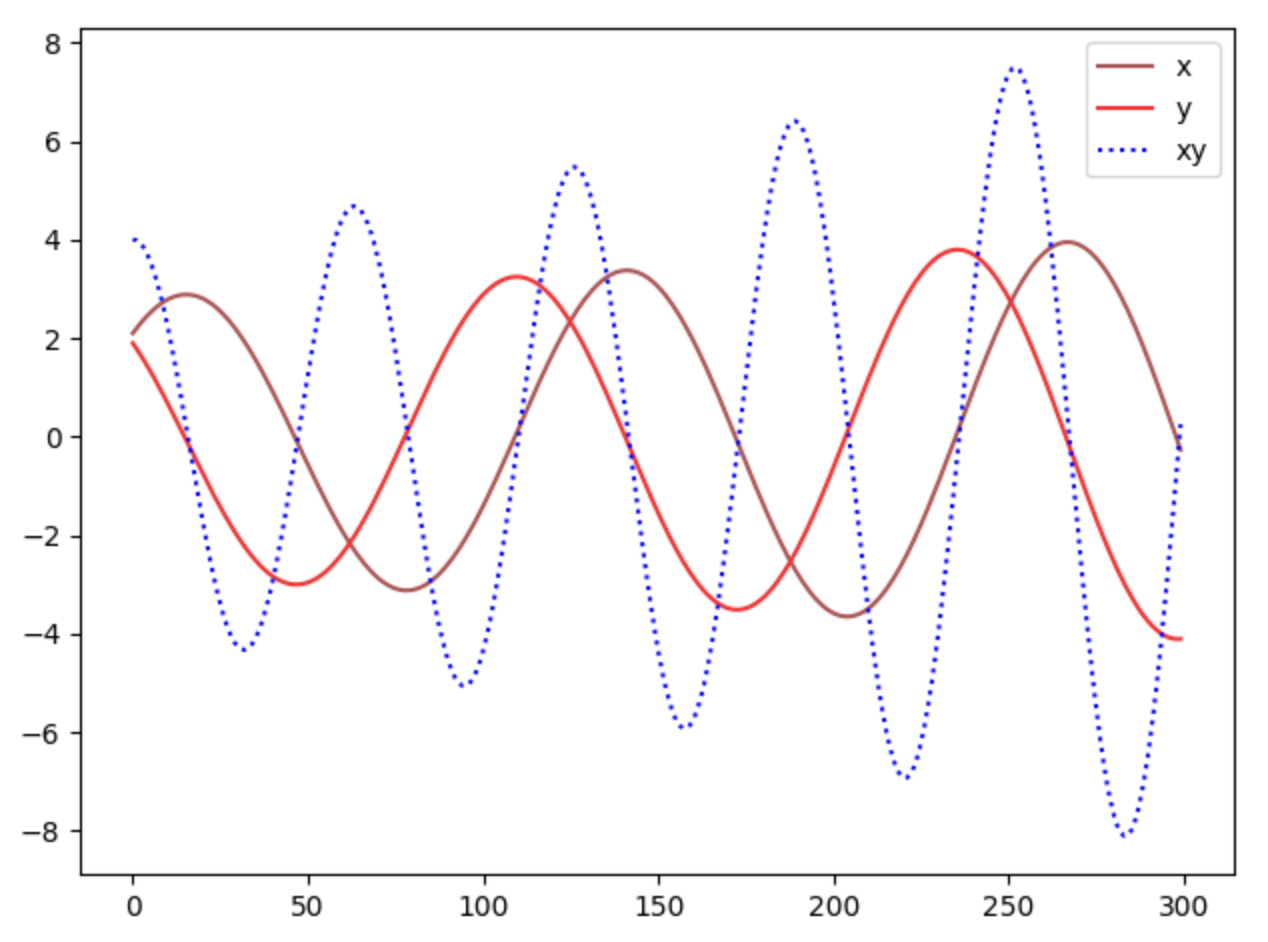
\includegraphics[width=5cm]{minmax4}
	\end{figure}
}

\frame{\frametitle{Non-convergence}
	\begin{itemize}
		\item If we increase the learning rate or train the model longer, we can see the parameters x, y is unstable with big swings.
	\end{itemize}
	\begin{figure}
		\centering
		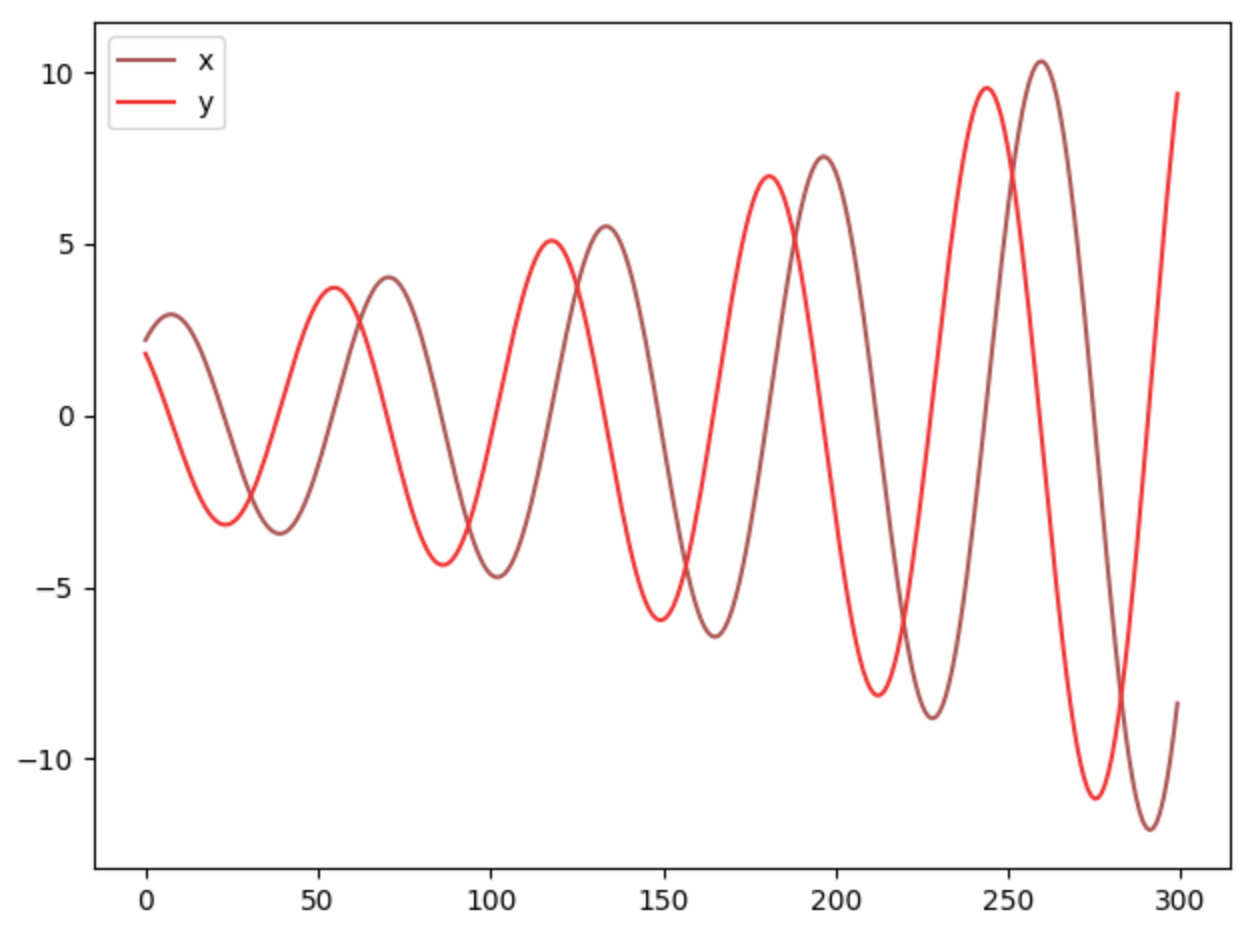
\includegraphics[width=5cm]{minmax5}
	\end{figure}
	\begin{itemize}
		\item Our example is an excellent showcase that \alert{some cost functions will not converge with gradient descent}, in particular for a non-convex game.
	\end{itemize}
}

\frame{\frametitle{Generative model with KL-Divergence}
	\begin{itemize}
		\item Before GAN, many generative models create a model θ that maximizes the Maximum Likelihood Estimation MLE. i.e. finding the best model parameters that fit the training data the most.
	\end{itemize}
	\begin{figure}
		\centering
		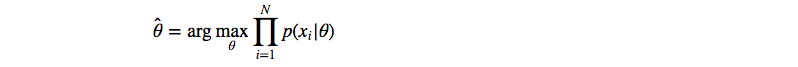
\includegraphics[width=9cm]{kl}
	\end{figure}
	\begin{itemize}
		\item KL $(x)$ drops to 0 for area where $p(x) → 0$. For example, in the figure on the right below, the red curve corresponds to $D(p, q)$. It drops to zero when $x>2$ where $p$ approaches 0.
	\end{itemize}
	\begin{figure}
		\centering
		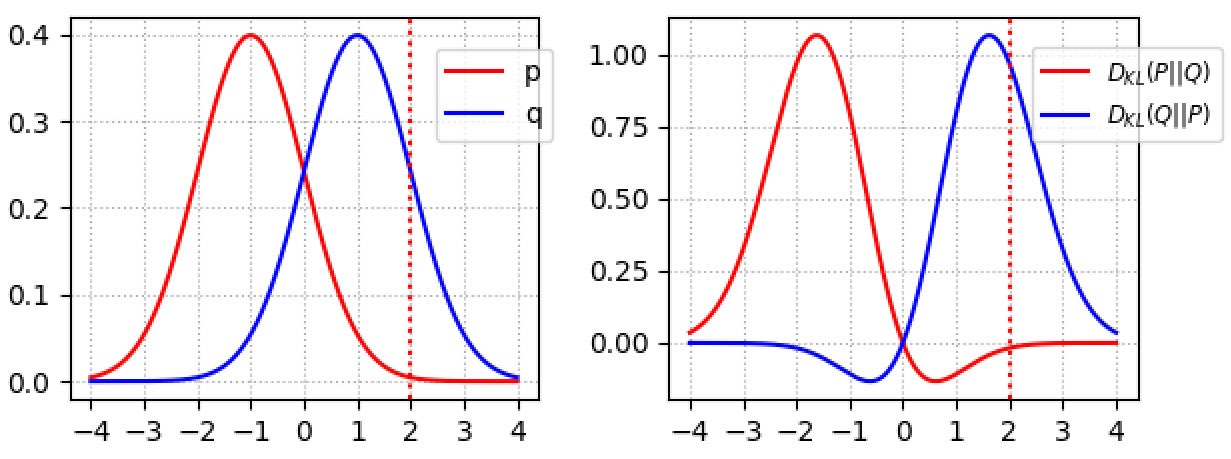
\includegraphics[width=6cm]{klchart}
		\caption{$KL(p, q)$ is the integral of the red curve in the right.}
	\end{figure}
}


\frame{\frametitle{Generative model with JL-Divergence}
	\begin{itemize}
		\item JS-divergence is defined as:
	\end{itemize}
	\begin{figure}
		\centering
		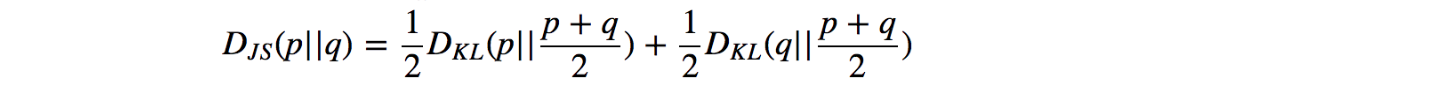
\includegraphics[width=9cm]{jl}
	\end{figure}
	\begin{figure}
		\centering
		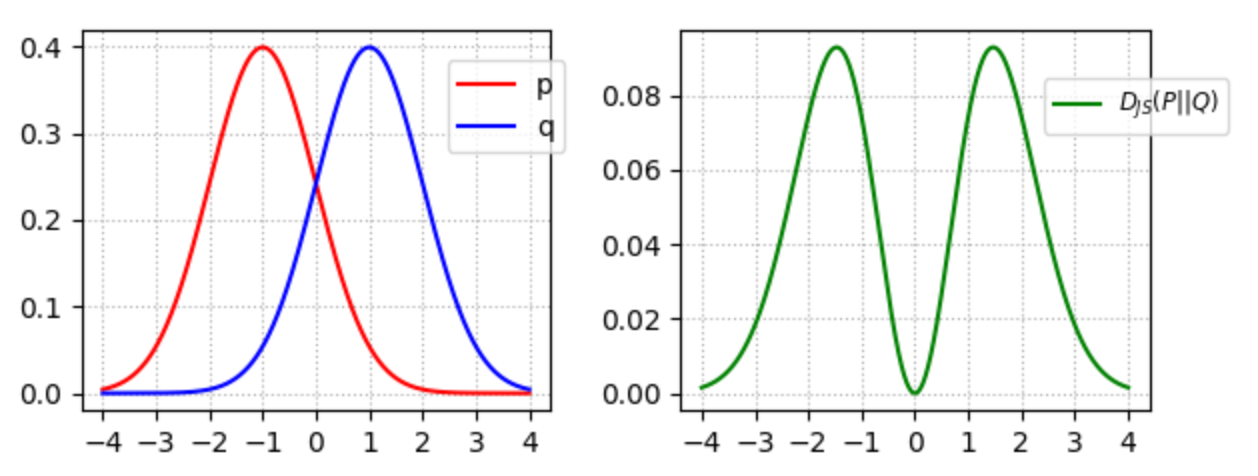
\includegraphics[width=6cm]{jlchart}
		\caption{$KL(p, q)$ is the integral of the red curve in the right.}
	\end{figure}
	\begin{itemize}
		\item JS-divergence is symmetrical.
		\item Unlike KL-divergence, it will penalize poor images badly.
		\item the generator’s objective function becomes:
	\end{itemize}
	\begin{figure}
		\centering
		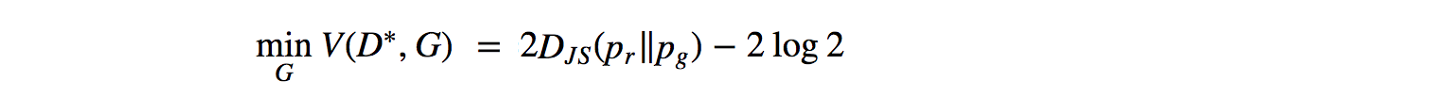
\includegraphics[width=9cm]{jl2}
	\end{figure}
}
